\documentclass[a4paper,12pt]{article}

\title{Physics 30 \\ Electric Forces \& Fields}
\author{Jad Chehimi}

% document setup
\renewcommand{\familydefault}{\sfdefault}
\linespread{1.25}
\usepackage[margin=1in]{geometry}
\usepackage{setspace}
\usepackage{enumitem}
\setlist{nosep}
\usepackage{color,soul}
\setcounter{secnumdepth}{0}

% tools
\usepackage[hidelinks]{hyperref}
\usepackage{float}
%% images
\usepackage{graphicx}
\graphicspath{ {./images/} }
%% science
\usepackage{siunitx}
\sisetup{exponent-product=\times, per-mode=fraction}

\begin{document}
\maketitle

% temp
\begin{center}
\Huge
Unfinished!
\normalsize
\end{center}
% temp

\tableofcontents

\pagebreak

\section{Electric Fields}
\begin{itemize}
    \item{Micheal Faraday: Developed the idea of "lines of force" to describe electric fields}
    \item{A field is a \hl{"sphere of influence"} in which a force can affect an object at a distance \hl{without contact}}
    \item{There are electric, gravitational, and magnetic fields}
    \item{The symbol for electric field is $|\vec{E}|$}
    \item{Do not mix this up with energy, which is scalar $\Delta{E}$}
\end{itemize}

\subsection{Gravitational Fields}
\Large $$\vec{g} = \SI{9.81}{\m\per\s\squared}$$ \normalsize

\Large $$\vec{g} = \frac{Gm}{r^2}$$ \normalsize
\begin{itemize}
    \item{$G$ = gravitational constant ($\SI{6.67e-11}{\N\cdot\m\squared\per\kg\squared}$)}
    \item{$m$ = mass of planet}
    \item{$r$ = radius of the planet}
\end{itemize}

$\vec{F}_g$ is ALWAYS attractive.

\pagebreak
\section{Drawing Electric Field Lines}
\begin{figure}[H]
    \centering
    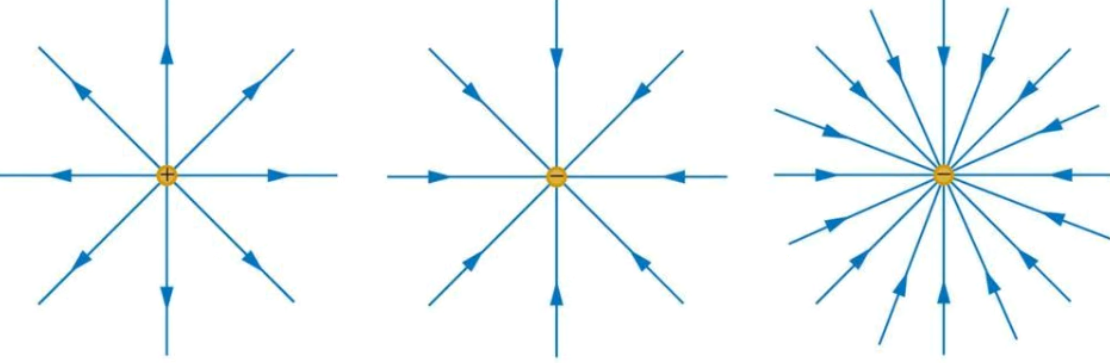
\includegraphics[width=0.75\textwidth]{fieldlines}
\end{figure}
\begin{itemize}
    \item{Like charges repel, opposite charges attract}
    \item{The field is stronger the closer to the source charge it is}
    \item{We \textbf{always} use a \hl{small positive test charge} to map/draw the electric field}
\end{itemize}

\subsection{Rules}
\begin{itemize}
    \item{The lines must originate on a positive charge and end on a negative charge (\hl{positive to negative})}
    \item{The electric field line must be \hl{perpendicular to the surface} of the charge}
    \item{The \hl{number of lines} drawn leaving a positive charge or approaching a negative charge is proportional to the \hl{magnitude of the charge}}
    \item{\hl{No two field lines can cross} each other}
\end{itemize}

\subsection{Electric Field Around A Positive v/s Negative Source Charge}
\begin{figure}[H]
    \centering
    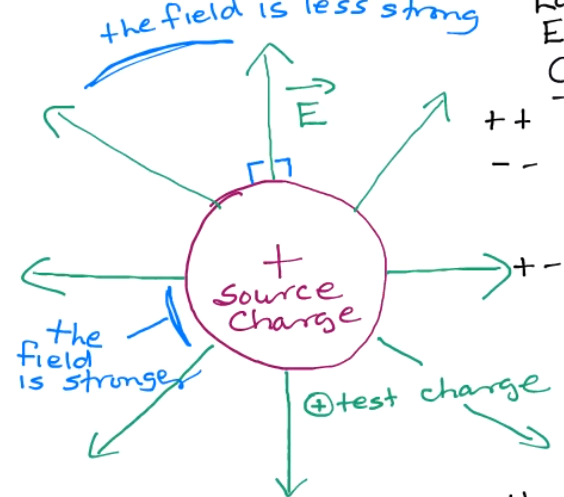
\includegraphics[width=0.4\textwidth]{lines}
    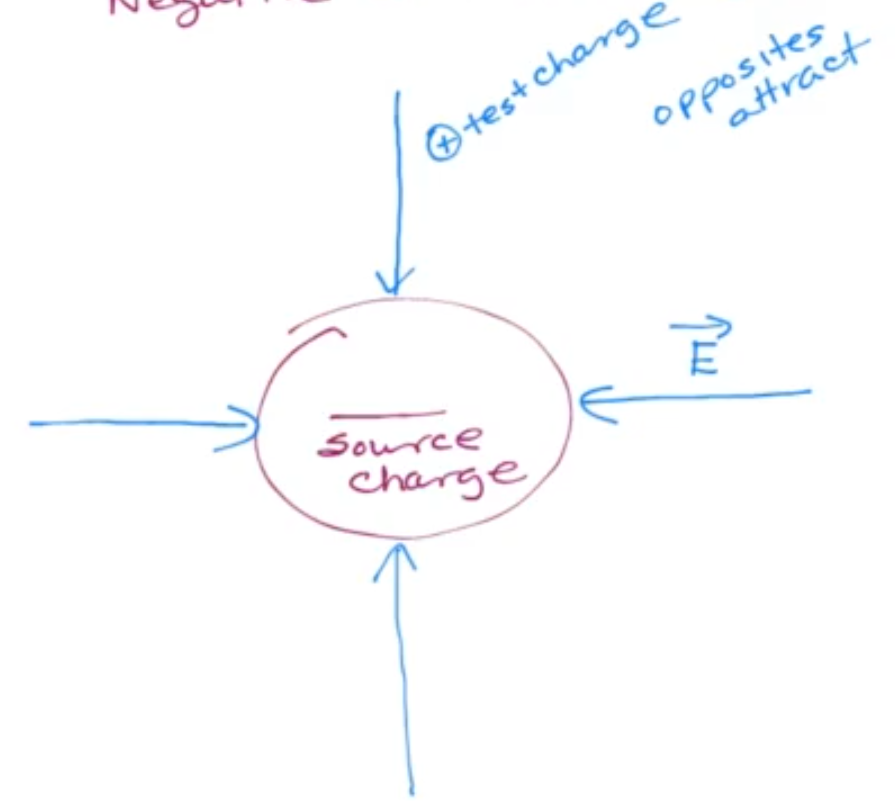
\includegraphics[width=0.4\textwidth]{lines2}
\end{figure}

\subsection{Electric Field Interactions}
\begin{figure}[H]
    \centering
    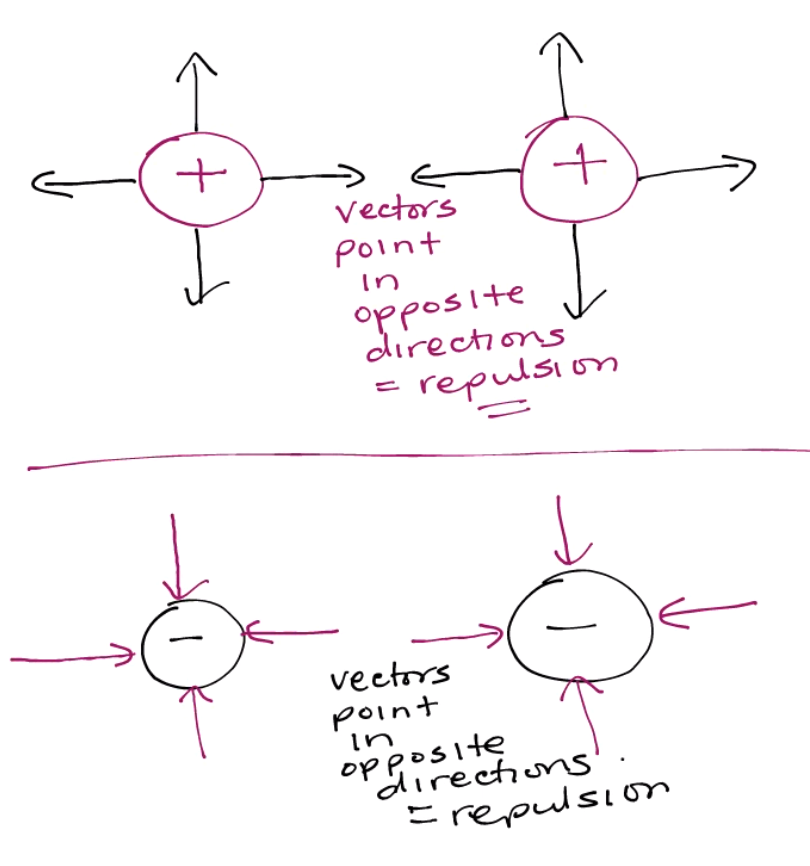
\includegraphics[width=0.4\textwidth]{repel}
    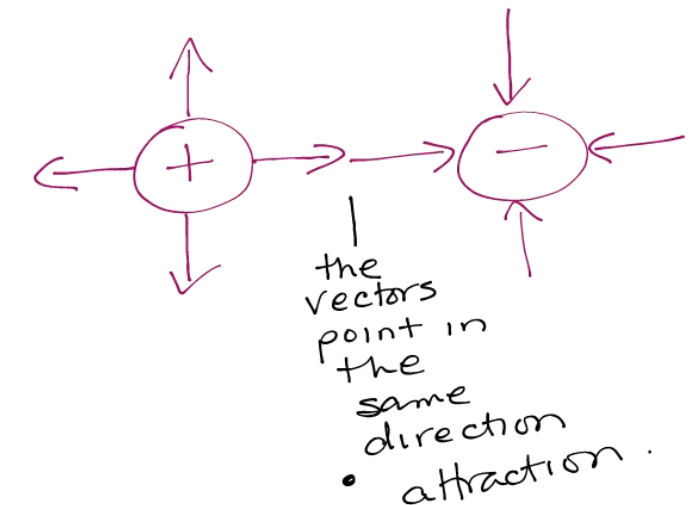
\includegraphics[width=0.4\textwidth]{attract}
\end{figure}

Use this theory with a test particle to determine the direction of an electric field. NOT signs.

For forces, NEVER use negatives for charges ($q$) in formulas. After you calculate a value with no negative charges, look at the signs. If they are same sign, the force is repel. If they are opposite sign, the force is attractive.

\section{Particles}
\begin{figure}[H]
    \centering
    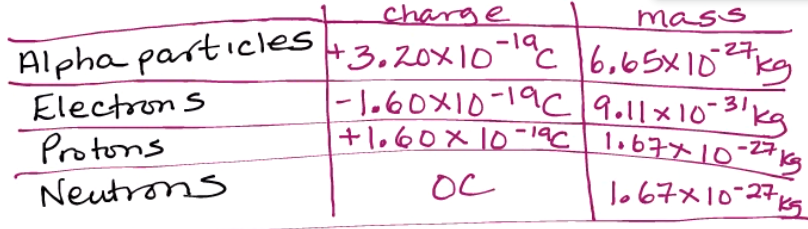
\includegraphics[width=\textwidth]{particles}
\end{figure}

\section{Electric Field Strength}
\subsection{Electric Field Around A Producer (Source Charge)}
\Large $$|\vec{E}| = \frac{kq}{r^2}$$ \normalsize
$$\textrm{Units: } \si{\newton\per\coulomb} \textrm{ or } \si{\V\per\m}$$
\begin{itemize}
    \item{$k$ = Coulomb's Constant (\SI{8.99e9}{\newton\cdot\m\squared\per\coulomb\squared})}
    \item{$q$ = Value of the source charge (\si{\coulomb})}
    \item{$r$ = Distance from the source charge (\si{\m})}
\end{itemize}

\subsection{Electric Field Experienced By A Charge}
\Large $$\vec{E} = \frac{\vec{F}_e}{q}$$ \normalsize
\begin{itemize}
    \item{$\vec{E}$ = Electric Field (\si{\newton\per\coulomb})}
    \item{$\vec{F}_e$ = Electrostatic Force (\si{\newton})}
    \item{$q$ = Test Charge (in a field question, its not source charge) (\si{\coulomb})}
\end{itemize}

\subsection{Example}
Calculate the electric field \SI{2.00}{\cm} from an alpha particle.
$$|\vec{E}| = \frac{(\SI{8.99e9}{\newton\cdot\m\squared\per\coulomb\squared})(\SI{3.20e-19}{\coulomb})}{(\SI{2.00e-2}{\m})^2}$$
$$|\vec{E}| = \SI{7.19e-6}{\newton\per\coulomb} \textrm{ radially outward}$$
\begin{figure}[H]
    \centering
    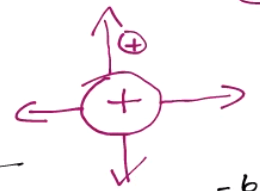
\includegraphics[width=0.3\textwidth]{fieldquestion}
\end{figure}

\subsection{Example II}
Calculate the electric field strength at a point in space where a \SI{3.24e-6}{\coulomb} charge experiences an electrostatic force of \SI{5.29e-3}{\newton}.
$$\vec{E} = \frac{\vec{F}_e}{q}$$
$$\vec{E} = \frac{\SI{5.29e-3}{\newton}}{\SI{3.24e-6}{\coulomb}}$$
$$\vec{E} = \SI{1.63e3}{\newton\per\coulomb}$$

\pagebreak
\subsection{Example III}
Calculate the electric field midway between the two charges below if they are \SI{5.00}{\cm} apart.
\begin{figure}[H]
    \centering
    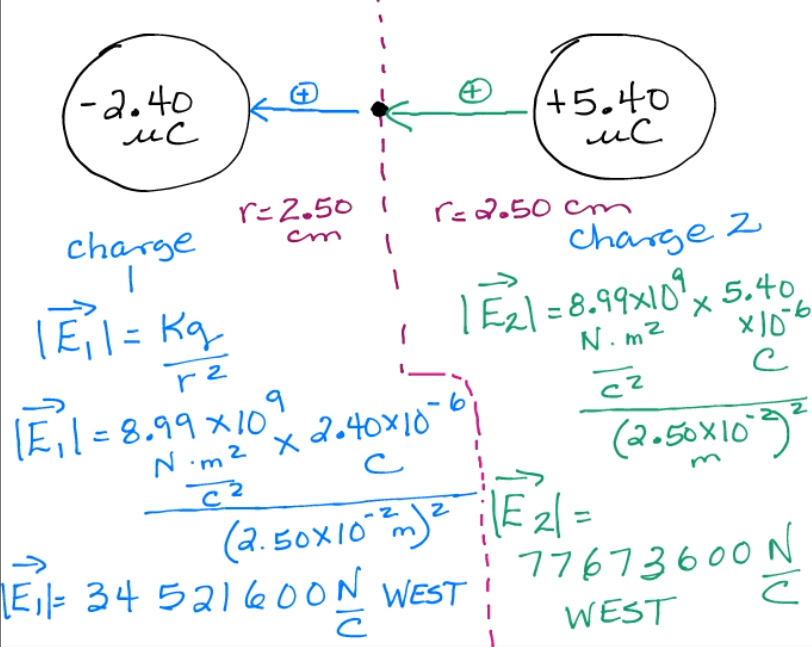
\includegraphics[width=\textwidth]{fieldquestion3}
\end{figure}

$$|\vec{E}_{net}| = |\vec{E}_1| + |\vec{E}_2|$$
$$|\vec{E}_{net}| = \SI{34521600}{\newton\per\coulomb}\textrm{, west} + \SI{77673600}{\newton\per\coulomb}\textrm{, west}$$
$$|\vec{E}_{net}| = \SI{1.12e8}{\newton\per\coulomb}\textrm{, west}$$

\pagebreak
\subsection{Electric Field Around A Producer in Two Dimensions}
\begin{itemize}
    \item{Calculate $\vec{E}$ of the hypotenuse}
    \item{Use trig to get the components of the electric field vector on each side}
\item{
    Direction of the vector is determined by the source charge like before
        \begin{itemize}
            \item{if positive, towards test charge/point (repel)}
            \item{if negative, from test charge/point to source charge (attract)}
        \end{itemize}
    }
    \item{Add the $x$ and $y$ components, positive or negative depending on direction}
    \item{You are left with the components of the net electric field vector}
\end{itemize}

\subsubsection{Example I}
\begin{figure}[H]
    \centering
    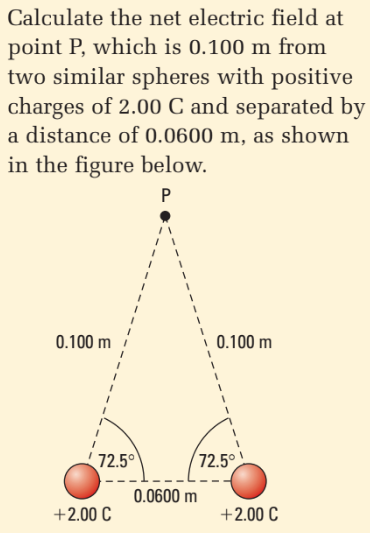
\includegraphics[width=0.6\textwidth]{fieldtriangle}
\end{figure}
$$= \SI{3.43e12}{\newton\per\coulomb}$$


\section{Electric Field Between Plates}
\Large $$\vec{E} = \frac{V}{d}$$ \normalsize
\begin{itemize}
    \item{$V$ = total voltage across the plate (\si{\volt})}
    \item{$d$ = total distance between the plates (\si{\meter})}
\end{itemize}

\begin{figure}[H]
    \centering
    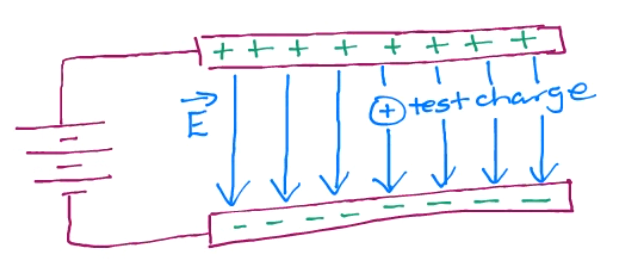
\includegraphics[width=0.50\textwidth]{plate}
\end{figure}

\begin{itemize}
    \item{The electric field between \hl{charged parallel plates} is \hl{uniform} --- identical at any point}
    \item{To determine the \hl{direction} of the electrical field between charged parallel plates, use a \hl{small positive test charge}}
    \item{
        Don't forget that \hl{work is equal to $\SI{0}{\joule}$} if the $F_e$ and $d$ are \hl{not along the same line}
        \begin{itemize}
            \item{$\theta$ (in $W = Fd\cos{\theta}$) must be either\\\ang{0} (force and distance same direction) or \\\ang{180} (force and distance opposite directions)}
        \end{itemize}
    }
\end{itemize}

\subsection{Example}
Two parallel plates are connected to a \SI{12.0}{\volt} battery. If the plates are \SI{6.00e-2}{\m} apart, calculate the electric field strength between them.
$$\vec{E} = \frac{\SI{12.0}{\volt}}{\SI{6.00e-2}{\m}} = \SI{200}{\volt\per\m}$$

\subsection{Example II}
\begin{figure}[H]
    \centering
    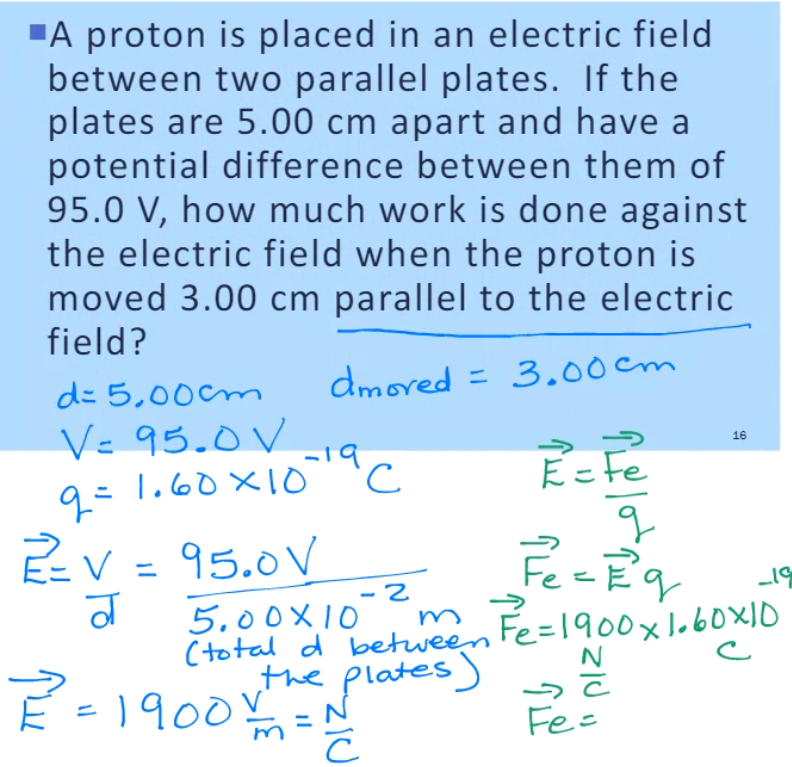
\includegraphics[width=0.39\textwidth]{workplate1}
    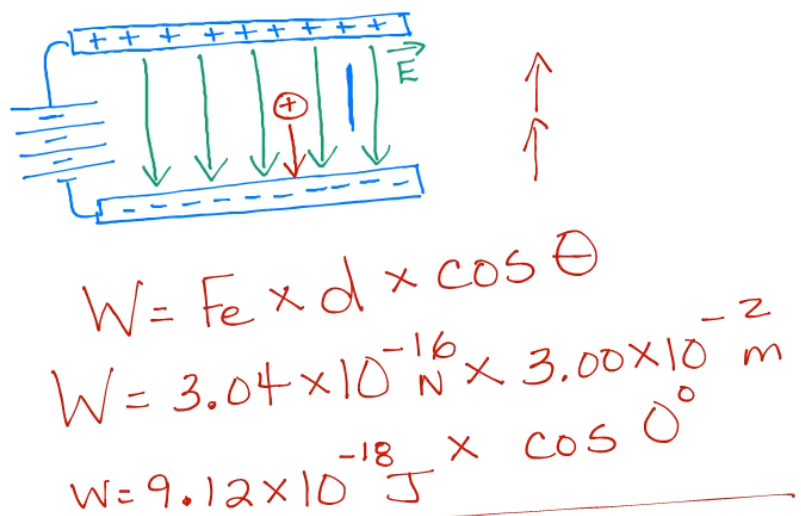
\includegraphics[width=0.5\textwidth]{workplate2}
\end{figure}

\subsection{Example III (Projectile Motion Style)}
An electron beam enters the region between two oppositely charged parallel plates near the negatively charged plate, as shown below. The plates are \SI{0.250}{\m} long and are \SI{0.0500}{\m} apart. There is an electrical potential difference of \SI{120}{\volt} across the two plates as the beam exits the region between the parallel plates. The path of the electrons just touches the edge of one of the plates as the beam exits the region between the parallel plates. \\Determine the minimum initial speed of an electron in the beam. \\Show the direction of the electric field and explain why.
\begin{figure}[H]
    \centering
    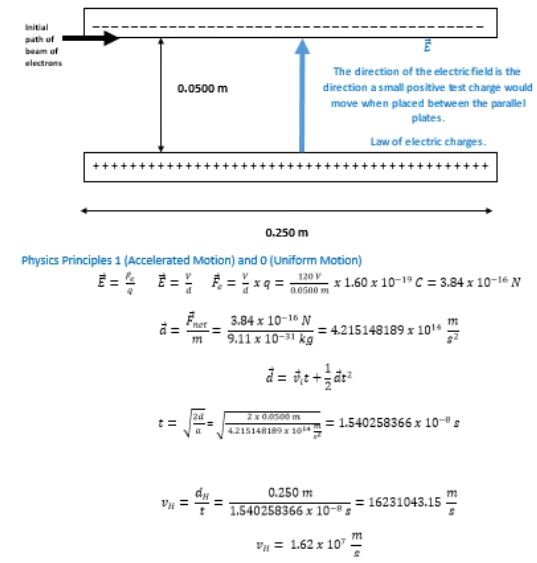
\includegraphics[width=\textwidth]{particleplates}
\end{figure}

\section{Electric Field as a Function of r Graph}
\begin{itemize}
    \item{Make sure all values are times ten to the power of the same exponent before you plot}
\end{itemize}

\begin{figure}[H]
    \centering
    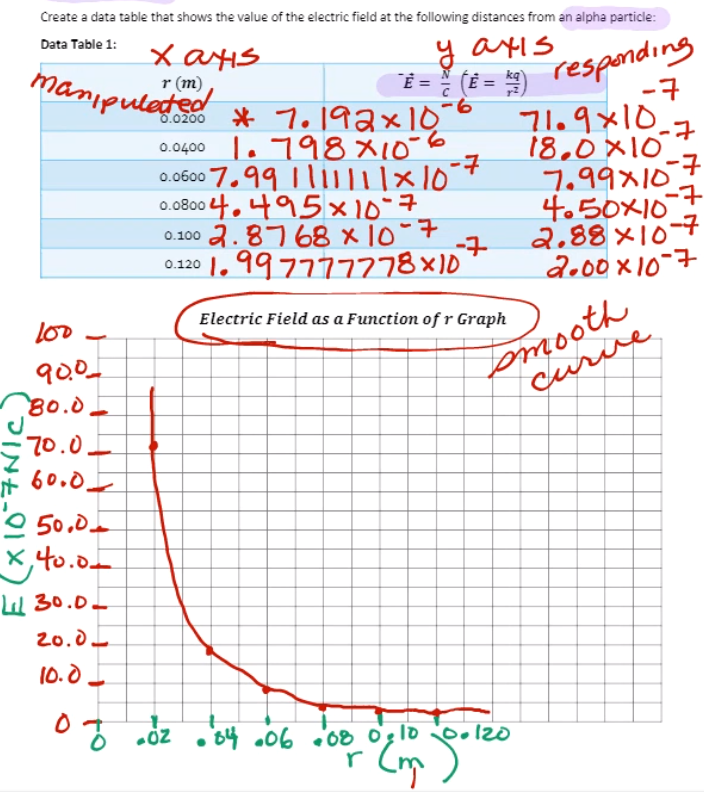
\includegraphics[width=0.75\textwidth]{graph1}
\end{figure}

In order to get a graph that is a straight line, set the $x$ to whatever is proportional to $y$. In this case, $E \propto \frac{1}{r^2}$

\begin{figure}[H]
    \centering
    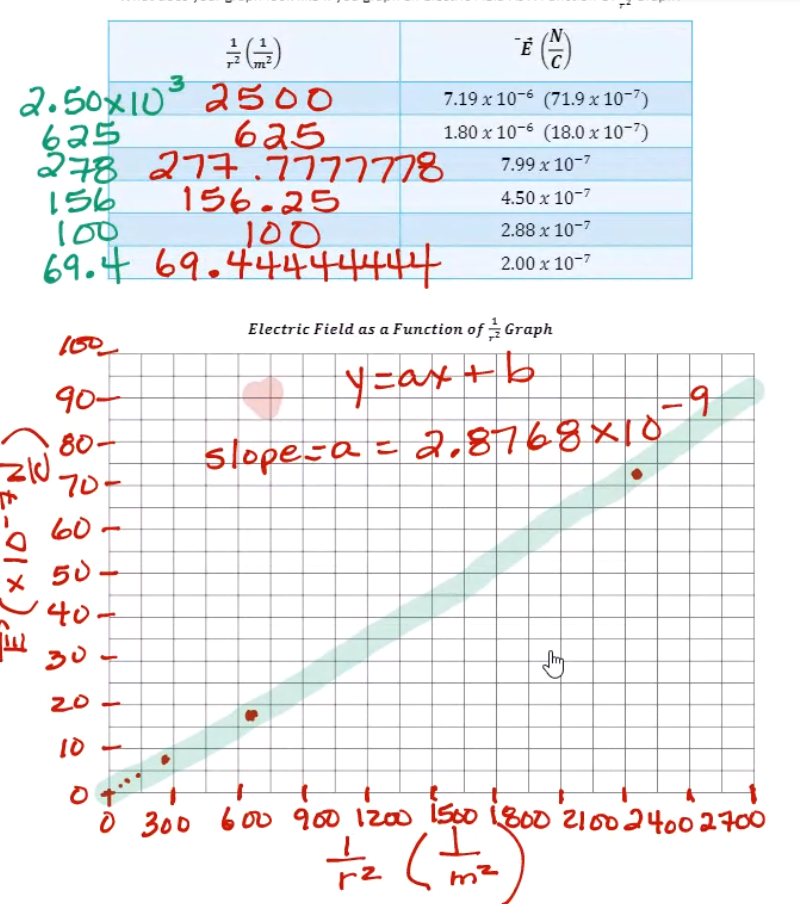
\includegraphics[width=0.75\textwidth]{graph2}
\end{figure}

Use the slope of this graph in further calculations.

slope = $\frac{E}{\frac{1}{r^2}} = Er^2$

You can substitute the slope into anywhere with $Er^2$.

These exact things also work for force as a function of separation distance graphs.\\$m = \frac{F}{\frac{1}{r^2}} = Fr^2$

\subsection{Slope}
Use your graphing calculator functions to calculate slope. (lists)

$$m = \frac{\Delta{y}}{\Delta{x}} = \frac{y_f - y_i}{x_f - x_i}$$

If you don't have a graphing calculator, manually calculate slope. Make sure to select points off the graph line that are \hl{not plotted points}.

\pagebreak
\section{Coulomb's Law}
\Large $$|\vec{F}_e| = \frac{kq_1q_2}{r^2}$$ \normalsize
$$F_e \propto q_1q_2 \qquad F_e \propto \frac{1}{r^2}$$

The magnitude of the electrostatic force of interaction between two point charges is directly proportional to the \textbf{scalar multiplication} of the magnitudes of charges and inversely proportional to the square of the distance between them.

Most questions are simply just plugging in the data you're given and solving for a variable.

\subsection{Data Miner Question}
\begin{itemize}
    \item{If two charges have \hl{brief contact}, the charges will evenly distribute}
    \item{Add the charges together and divide by two}
    \item{Both will share this new charge if the objects are same size and material, which it always will be at the Physics 30 level}
    \item{Some questions ask for the speed/acceleration of charged objects. For these questions, remember that $F_e = F_c$, and $F_c = ma_c$ (which is on your formula sheet) (this doesn't apply to parallel plates questions)}
\end{itemize}

\subsubsection{Example}
A \SI{7.50}{\micro\coulomb} charge and a \SI{-9.24}{\micro\coulomb} charge are brought into \textbf{brief contact}, then moved \SI{1.75}{\cm} away from each other. Calculate the electrostatic force between the two charges.
$$\SI{7.50e-6}{\coulomb} + \SI{-9.24e-6}{\coulomb} = \SI{-1.74e-6}{\coulomb}$$
$$\SI{-1.74e-6}{\coulomb} \div 2 = \SI{-8.70e-7}{\coulomb}$$

$$|\vec{F}_e| = \frac{(\SI{8.99e9}{\newton\cdot\m\squared\per\coulomb\squared})(\SI{8.70e-7}{\coulomb})(\SI{8.70e-7}{\coulomb})}{(\SI{1.75e-2}{\m})^2}$$
$|\vec{F}_e| = \SI{22.2}{\newton} \textrm{ repulsive}$ (like charges repel)

\subsection{Long Answer Example}
An electron and a proton in the hydrogen atom are separated by \SI{5.29e-11}{\m} when the electrion is in the first Bohr orbit.
\\a) Calculate $\vec{F}_g$ between the electron and proton.
\\b) Calculate $\vec{F}_e$ between the electron and proton.
\\c) Which force, $\vec{F}_g$ or $\vec{F}_e$, is responsible for the electron orbiting the nucleus? Why?
\\d) Calculate the speed of the electron as it orbits the nucleus.
\\e) Calculate the period of the electron.

\begin{figure}[H]
    \centering
    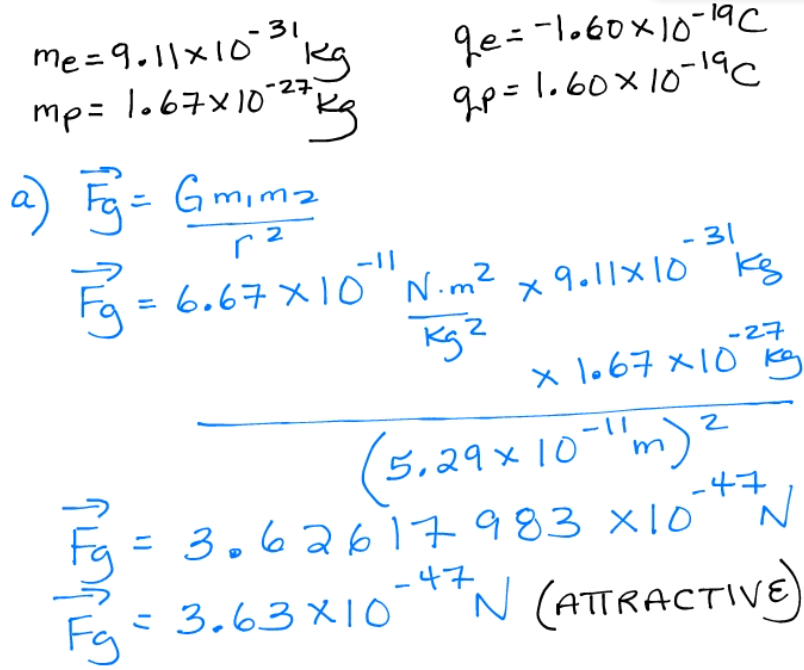
\includegraphics[width=0.45\textwidth]{longa}
    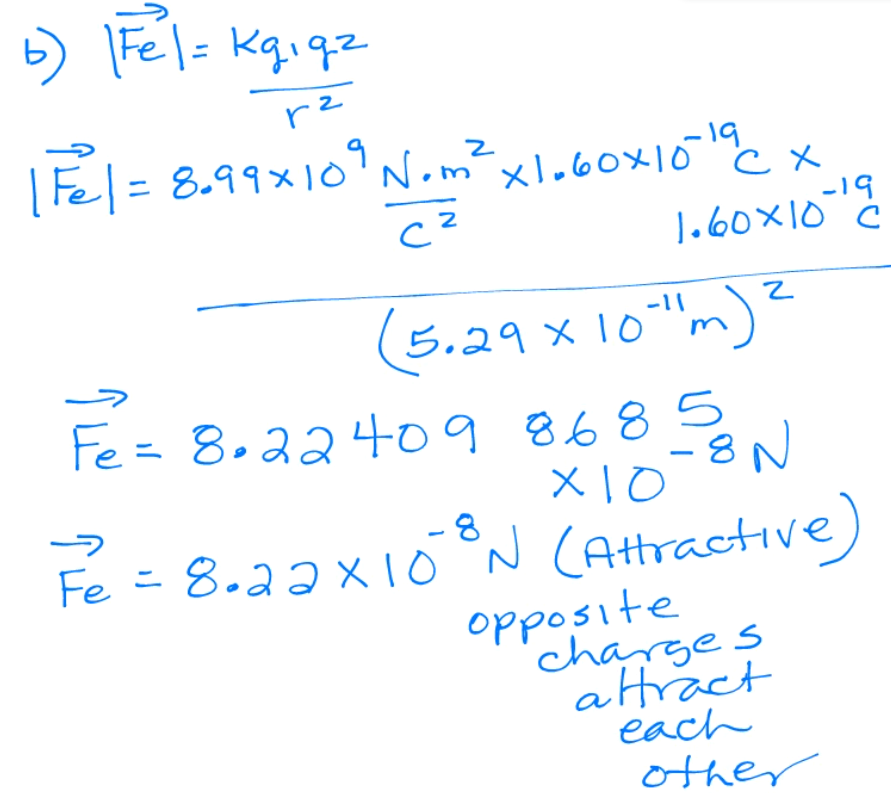
\includegraphics[width=0.45\textwidth]{longb}
\end{figure}
c) $\vec{F}_e$ is responsible for the electron's orbit as it is significantly larger than $\vec{F}_g$.
\begin{figure}[H]
    \centering
    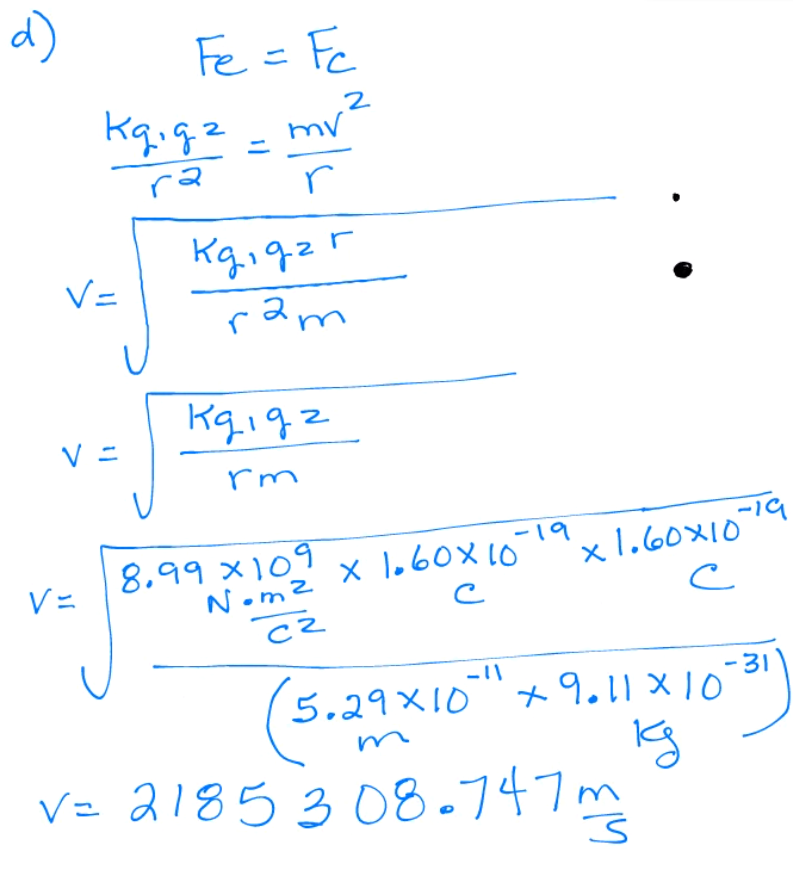
\includegraphics[width=0.45\textwidth]{longd}
    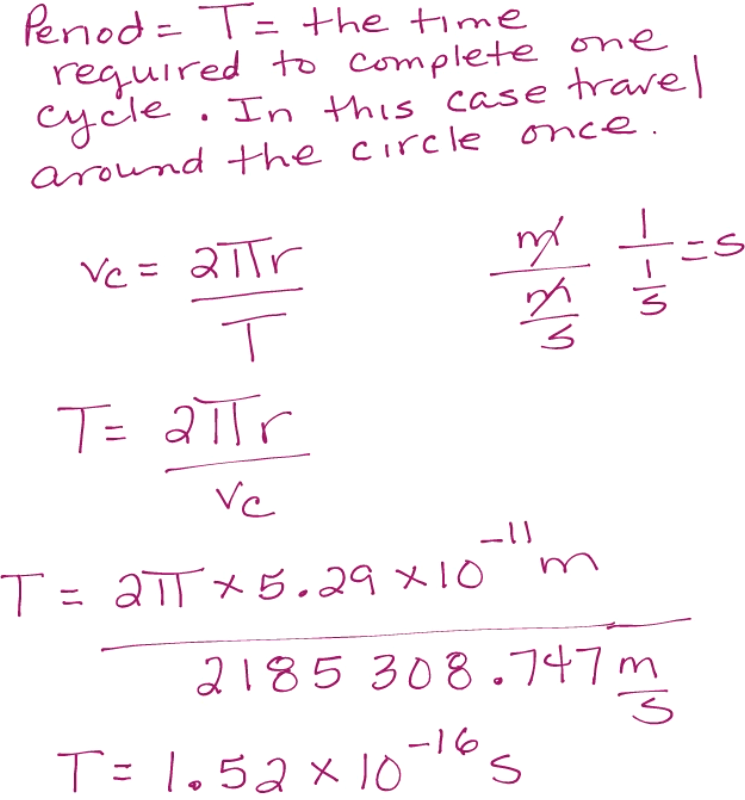
\includegraphics[width=0.45\textwidth]{longe}
\end{figure}

\pagebreak
\subsection{Multiple Charges Example}
Calculate the $F_e$ exerted on charge B due to charges A and C.
\begin{figure}[H]
    \centering
    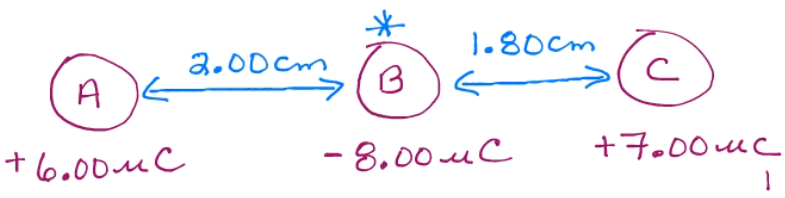
\includegraphics[width=0.50\textwidth]{Fequestion}
\end{figure}
\begin{figure}[H]
    \centering
    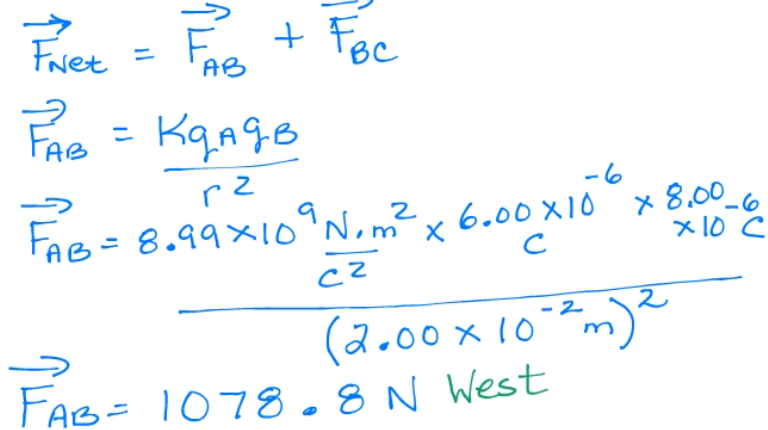
\includegraphics[width=0.45\textwidth]{Fequestion2}
    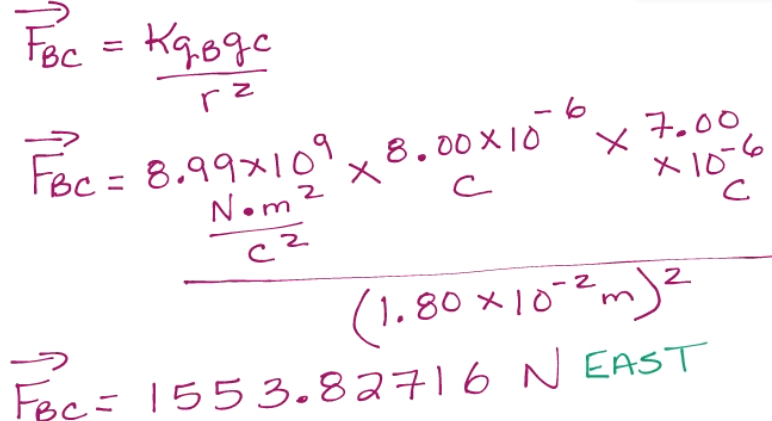
\includegraphics[width=0.45\textwidth]{Fequestion3}
    \caption{The direction of each force is where the reference charge (charge B) is going to move. \\For instance, A and B are opposite charges, they'll attract. A is on the west of B, so the force is west.}
    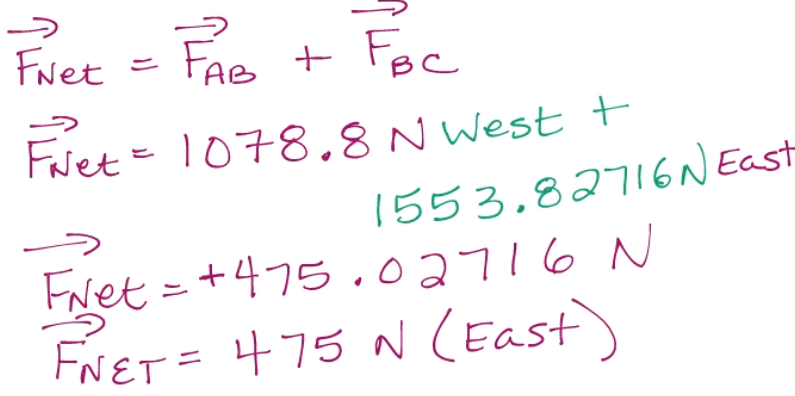
\includegraphics[width=0.75\textwidth]{Fequestion4}
\end{figure}

\subsection{Multiple Charges Example I}
\begin{figure}[H]
    \centering
    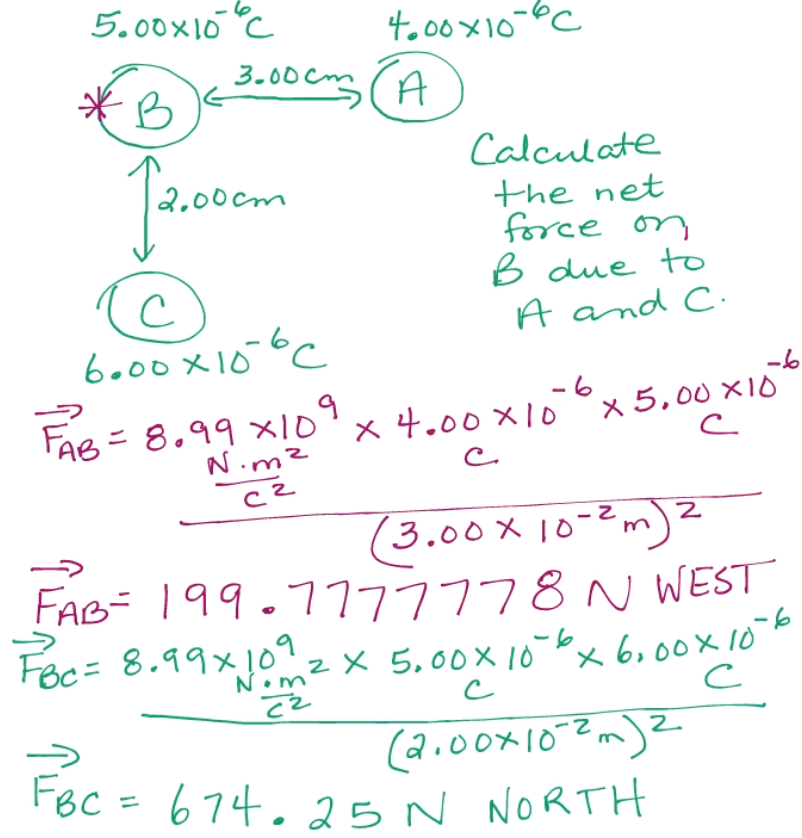
\includegraphics[width=0.7\textwidth]{multiple}
    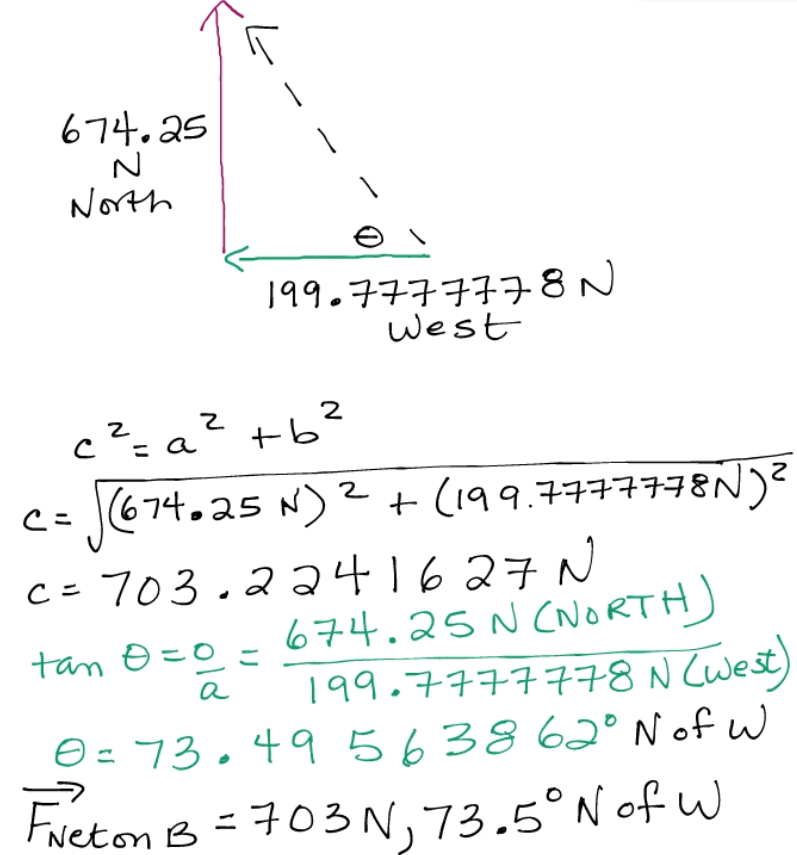
\includegraphics[width=0.7\textwidth]{multiple2}
\end{figure}

\section{Electronvolts}
Energy can be measured in Joules or in electronvolts. (\si{\electronvolt})

If you need to calculate speed, energy must be in Joules. (\si{\joule})

On your data sheet, it says \hl{$\SI{1}{\electronvolt} = \SI{1.60e-19}{\joule}$}

\section{Voltage (Potential Differnece)}
$$V = \frac{\Delta{E}}{q}$$
$$\textrm{Unit} = \si{\volt} = \si{\joule\per\coulomb}$$

If you apply a voltage to a charge, the charge will experience a change in energy.

\subsection{Example}
An electron is accelerated by a potential difference of \SI{20000}{\volt} in a cathode ray tube television. Calculate the change in energy experienced by the electron. Calculate the speed of the electron.

$$\Delta{E} = \SI{20000}{\volt} \times \SI{1.60e-19}{\coulomb}$$
$$\Delta{E} = \SI{3.20e-15}{\joule}$$

\begin{figure}[H]
    \centering
    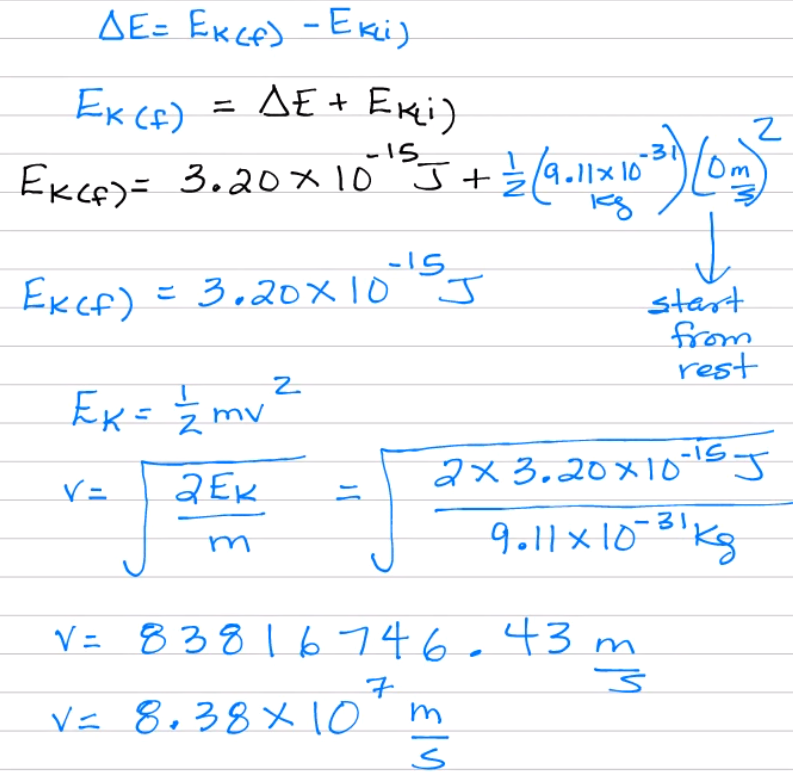
\includegraphics[width=0.5\textwidth]{voltage}
\end{figure}

\subsection{Example II}
\begin{figure}[H]
    \centering
    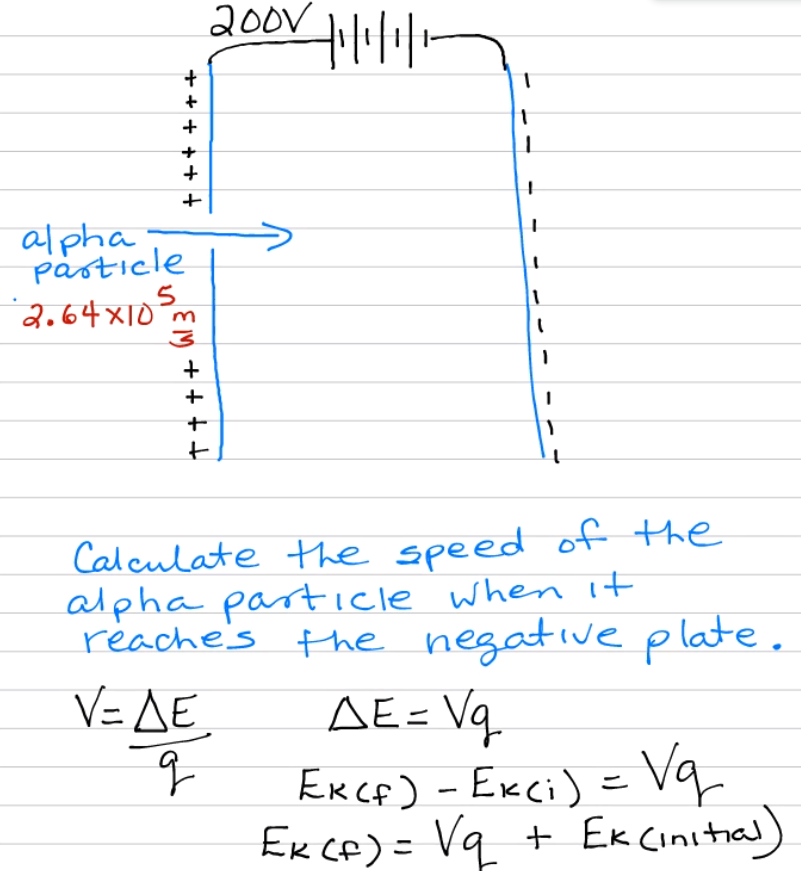
\includegraphics[width=0.60\textwidth]{voltspeed1}
    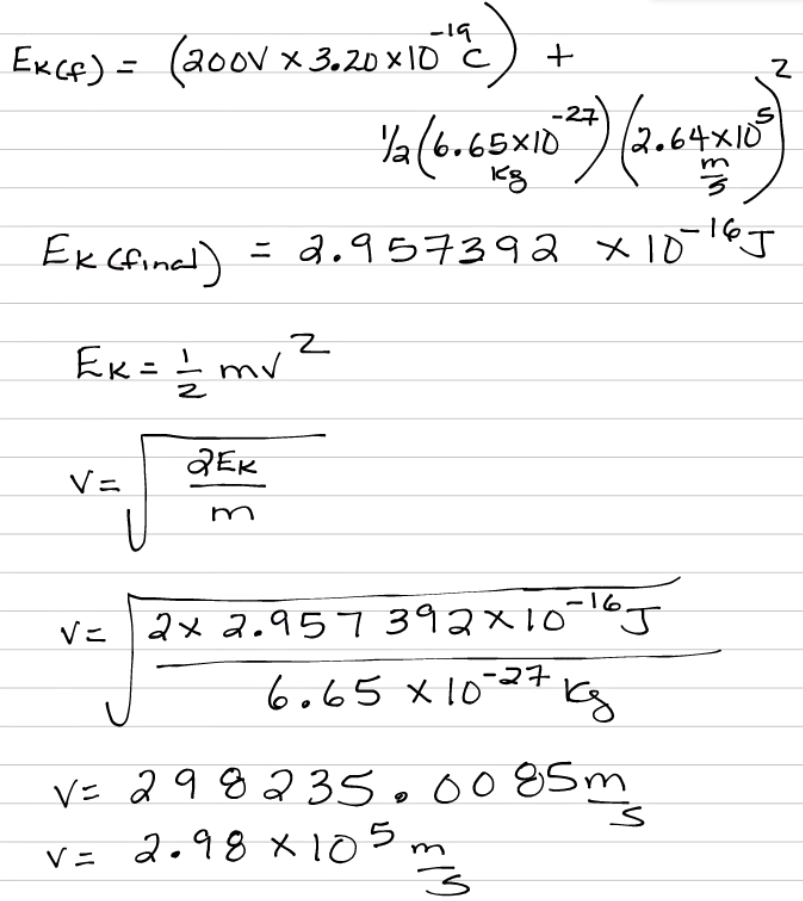
\includegraphics[width=0.60\textwidth]{voltspeed2}
\end{figure}

\section{Millikan Oil Drop Experiment}
\begin{itemize}
    \item{
        Millikan discovered...
        \begin{itemize}
            \item{charge is quantized (charge has a discrete amount)}
            \item{the elementary charge ($e = \SI{1.60e-19}{\coulomb}$)}
        \end{itemize}
    }
\end{itemize}

Millikan made use of the uniform electric fields in the region between two oppositely charged parallel plates. He charged the plates by connecting each to opposite terminals of a large bank of storage batteries whose potential difference could be varied. He called this apparatus an electrical microbalance. He was able to isolate and suspend charged oil drops, and ultimately measure the charge on each oil drop.

\begin{figure}[H]
    \centering
    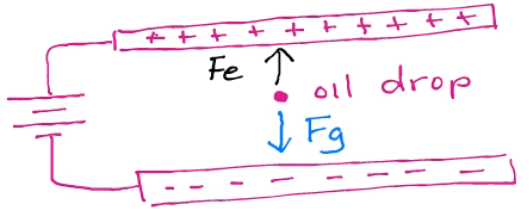
\includegraphics[width=0.50\textwidth]{oil}
\end{figure}
\subsection{Millikan Equation}
\Large $$\vec{F}_{net} = \vec{F}_e + \vec{F}_g$$ \normalsize

To suspend an oil drop between plates, the electrostatic force must be equal and opposite to the force of gravity. Therefore, if the \hl{oil drop is suspended, $F_{net} = \SI{0}{\newton}$}, since theres zero acceleration. (this also applies to the drop being in uniform motion, also zero acceleration)

\Large $$\vec{F}_g = \vec{F}_e$$ \normalsize
This is a shortcut to the above equation if $\vec{F}_{net}$ is zero --- suspended oil drop. The reason the force of gravity isn't negative is because it was cancelled by gravity being negative. ($\vec{F}_g = m(\SI{-9.81}{\m\per\s\squared})$)

\subsection{Miscellaneous Equations (memorize)}
$$\textrm{Volume of a sphere} = \frac{4}{3}\pi r^3$$
$$\textrm{density} = \frac{\textrm{mass}}{\textrm{volume}}$$

\subsubsection{Charge to Electrons}
\Large$$n = \frac{q}{e}$$\normalsize
\begin{itemize}
    \item{$n$ = number of electrons}
    \item{$q$ = charge (\si{\coulomb})}
    \item{$e$ = elementary charge (\SI{1.60e-19}{\coulomb})}
\end{itemize}

\subsection{Example}
An oil drop with a mass of \SI{7.32e-15}{\kg} is suspended between two parallel plates that are \SI{6.50}{\milli\m} apart. If the potential difference between these plates is \SI{650}{\volt}, how many excess electrons does this oil drop carry?
\begin{itemize}
    \item{$m = \SI{7.32e-15}{\kg}$}
    \item{$\vec{a} = \SI{0}{\m\per\s\squared}$ (suspended)}
    \item{$d = \SI{6.50e-3}{\m}$}
    \item{$V = \SI{650}{\volt}$}
    \item{$g = \SI{9.81}{\m\per\s\squared}$}
\end{itemize}
$$\vec{E} = \frac{V}{d} = \frac{\SI{650}{\volt}}{\SI{6.50e-3}{\m}} = \SI{100000}{\volt\per\m} \textrm{ or } \si{\newton\per\coulomb}$$
$$\vec{F}_{net} = \vec{F}_e + \vec{F}_g \quad\longrightarrow\quad m\vec{a} = \vec{E}q + m\vec{g}$$
$$q = \frac{m\vec{a} - m\vec{g}}{\vec{E}}$$
$$q = \frac{0 - (\SI{7.32e-15}{\kg})(\SI{-9.81}{\m\per\s\squared})}{\SI{100000}{\newton\per\coulomb}} = \SI{7.18e-19}{\coulomb}$$
$$\frac{\num{1}\textrm{ electrons}}{\SI{1.60e-19}{\coulomb}} = \frac{n\textrm{ electrons}}{\SI{7.18e-19}{\coulomb}} \textrm{ or use } n = \frac{q}{e}$$

$n = \num{4.488075}\textrm{ electrons} = \num{4}\textrm{ electrons}$ (electrons cannot be fractional, so round down)

\subsection{Example II}
An oil drop weighs \SI{9.24e-15}{\newton}. If it is suspended between two horizontal plates where the electric field strength is \SI{4500}{\newton\per\coulomb}, what is the magnitude of the charge on the oil drop?
\begin{itemize}
    \item{$F_g = \SI{9.24e-15}{\newton}$}
    \item{$\vec{E} = \SI{4500}{\newton\per\coulomb}$}
\end{itemize}
$$\vec{F}_g = \vec{F}_e = \vec{E}q$$
$$q = \frac{\vec{F}_g}{\vec{E}} = \SI{2.05e-18}{\coulomb}$$

\pagebreak
\subsection{Example III}
An oil drop whose mass is \SI{3.67e-15}{\kg} accelerates downward at a rate of \SI{2.75}{\m\per\s\squared} when placed between two horizontal plates that are \SI{2.50}{\centi\m} apart. The potential difference between the plates is \SI{1000}{\volt}. Assuming the oil drop is negative and the top plate is positive, what is the charge on this oil drop?
\begin{itemize}
    \item{$m = \SI{3.67e-15}{\kg}$}
    \item{$g = \SI{-9.81}{\m\per\s\squared}$}
    \item{$a = \SI{-2.75}{\m\per\s\squared}$}
    \item{$d = \SI{2.50e-2}{\m}$}
    \item{$V = \SI{1000}{\volt}$}
\end{itemize}
$$\vec{F}_{net} = \vec{F}_e + \vec{F}_g$$
$$m\vec{a} = \vec{E}q + m\vec{g}$$
$$q = \frac{m\vec{a} - m\vec{g}}{\frac{V}{d}} = \SI{6.48e-19}{\coulomb}$$

\subsection{Example IV (No Mass Given)}
In a Millikan Oil Drop experiment, a student sprayed oil droplets with a density of \SI{827}{\kg\per\m\cubed} between two horizontal parallel plates that were \SI{5.20}{\centi\m} apart. The student adjusted the potential difference between the plates to ber \SI{5500}{\volt} so that one of the drops becomes stationary. The diameter of this drop was measured to be \SI{4.24e-6}{\m}. Calculate the magnitude of the charge on this oil droplet.
\begin{itemize}
    \item{density = \SI{827}{\kg\per\m\cubed}}
    \item{$d = \SI{5.20e-2}{\m}$}
    \item{$V = \SI{5500}{\volt}$}
    \item{$r = \SI{2.12e-6}{\m}$}
\end{itemize}

$$\textrm{Volume of a sphere} = \frac{4}{3}\pi r^3 = \SI{3.99e-17}{\m\cubed}$$
$$\textrm{mass} = \textrm{density} \times \textrm{volume} = (\SI{827}{\kg\per\m\cubed})(\SI{3.99e-17}{\m\cubed}) = \SI{3.30e-14}{\kg}$$
Solve the rest like usual, now that you have mass, $q = \SI{3.06e-18}{\coulomb}$

\pagebreak
\section{Charging Objects}
There are three ways an object can be charged, and in each only the electrons move. The protons stay in the nucleus.
\begin{itemize}
    \item{Friction}
    \item{Conduction}
    \item{Induction}
\end{itemize}

\subsection{Friction}
Charging by friction occurs when electrons are "wiped" from one object onto another. e.g. rubbing

\subsection{Conduction}
Charging by conduction occurs when electrons move from one object to another through \hl{direct contact}.

\begin{figure}[H]
    \centering
    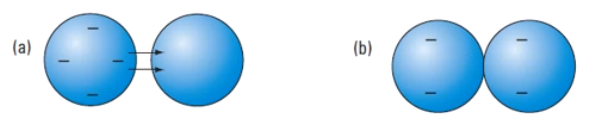
\includegraphics[width=0.50\textwidth]{conduction}
\end{figure}

\subsubsection{Grounding}
The process of transferring charge to and from Earth. Conductive path to Earth.

\begin{figure}[H]
    \centering
    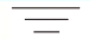
\includegraphics[width=0.1\textwidth]{ground}
\end{figure}

\subsection{Induction}
Charging by induction occurs when charges in an uncharged object are rearranged \hl{without direct contact} with a charged object.

e.g. If you charge a balloon through friction and place the balloon near paper, the charges of the paper will be rearranged and the paper will be attracted to the balloon.

\textbf{Charge Migration}: Movement of electrons in a neutral object where one side of the object becomes positive and the other side becomes negative.

\textbf{Separation of Charge}: Bringing a charged object near a neutral one will cause a separation of charge.

\begin{figure}[H]
    \centering
    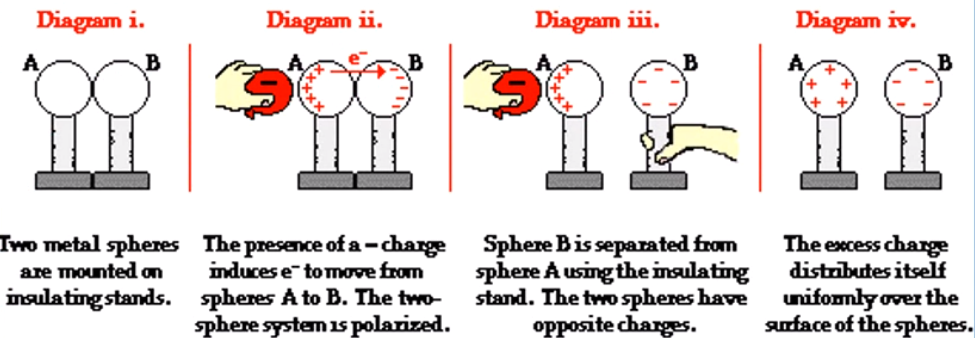
\includegraphics[width=0.75\textwidth]{induction}
\end{figure}

\section{Conservation of Charge}
When you charge something by any method, \hl{no charges are created or destroyed}.

The number of electrons and protons in the entire system is constant. Electrons move from one atom to another.

\section{Materials}
\subsection{Insulator}
\begin{itemize}
    \item{Electrons are tightly bound to the nucleus}
    \item{Electrons are not free to move within the substance}
    \item{e.g. plastic, rubber, glass, wood, air}
\end{itemize}

\subsection{Conductor}
\begin{itemize}
    \item{Electrons are in the outermost regions of atom}
    \item{Electrons are free to move}
    \item{e.g. copper, aluminum, mercury}
\end{itemize}

\section{Static Electricity}
\begin{itemize}
    \item{The electric charge at rest on an object}
    \item{When something is static, it is not moving}
    \item{The charges of static electricity do not move away from the object that they are in, so the object keeps its charge}
\end{itemize}

\section{How Lightning Forms}
During a thunderstorm, water droplets, ice, and air move inside the storm cloud. As a result, negative charges build up, often at the bottom of the cloud. Positive charges often build up at the top.

The negative charge at the bottom of the cloud may induce a positive charge on the ground. The large charge difference causes a rapid electric discharge called lighting.

Different parts of clouds have different charges. In fact, most lighting happens within and between clouds.

\section{Electric Current}
Electric current is the rate of flow of electrons.
\Large $$I = \frac{q}{t}$$ \normalsize
\begin{itemize}
    \item{$I$ = current (amps, \si{\ampere} = \si{\coulomb\per\s})}
    \item{$q$ = charge (\si{\coulomb})}
    \item{$t$ = time (\si{\s})}
\end{itemize}

\subsection{Example}
A circuit has a constant current of \SI{6.00}{\ampere}, in one second how many electrons will travel through a light bulb in that circuit?
$$It = q$$
$$(\SI{6.00}{\ampere})(\SI{1}{\s}) = \SI{6.00}{\coulomb}$$

$$n = \frac{q}{e}$$
$$n = \frac{\SI{6.00}{\coulomb}}{\SI{1.60e-19}{\coulomb}} = \num{3.75e-19}\textrm{ electrons}$$

\section{Pith Ball Hanging from an Insulating Thread}
\begin{figure}[H]
    \centering
    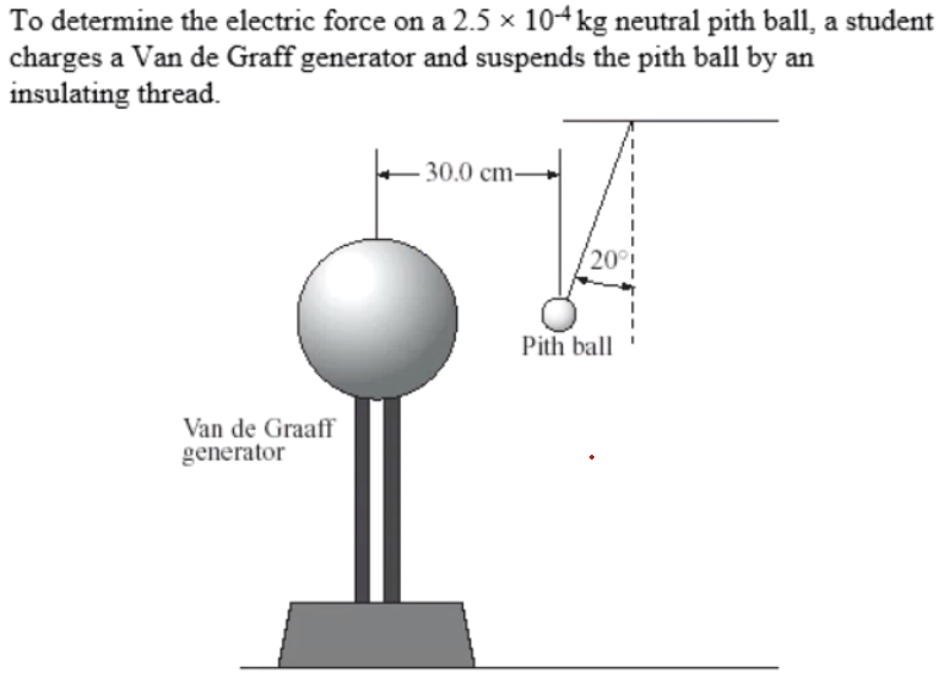
\includegraphics[width=0.8\textwidth]{pith}
\end{figure}

When the neutral pith ball is placed near the charged Van de Graff generator, the pith ball is attracted to the generator as a result of \hl{induction}.

The direction of the electrical force on the pith ball is \hl{left}.

\begin{figure}[H]
    \centering
    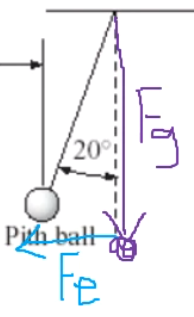
\includegraphics[width=0.15\textwidth]{pithforces}
\end{figure}
$$\tan{\theta} = \frac{F_e}{F_g}$$
$$F_g\tan{\theta} = F_e$$
$$F_g = mg = \SI{2.45e-3}{\newton}$$
$$\num{2.45e-3}\tan{\ang{20}} = F_e$$
$$\SI{8.9e-4}{\newton} = F_e$$

\end{document}
